\section{Traditional Approaches}

Determining the chromatic number of a graph is of a class of problems called \emph{NP-hard}.

\subsection{Runtime Complexity}

\subsection{Lower Bound}

\subsection{Upper Bound}

\subsection{Zykov Algorithms}

An exhaustive, exponential-time algorithm for determining the chromatic number of a graph is derived from a
nondeterministic Turing machine technique attributed to Ukranian graph theorist Alexandre A. Zykov (1922--2013)
\cite{obit}.

\begin{figure}[h]
  \label{fig:zykov}
  \begin{center}
    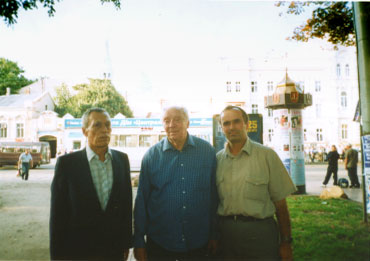
\includegraphics{photo}
  \end{center}
  \caption{V.G Vizing (L), A.A. Zykov (C), and V.I. Voloshin (R) in Odessa (2001) \cite{voloshin}}
\end{figure}

\subsubsection{The Chromatic Polynomial}

In his 1949 paper (translated by the AMS in 1952) \cite{zykov}, Zykov addresses the question: given a graph \(G\) and
a number \(k\in\N\), how many ways are there to properly color \(G\) using at most \(k\) colors?  In fact, he is not
particularly concerned about the chromatic number, which he calls the \emph{rank}, of a graph.  To solve this problem,
Zykov notes that in any proper coloring of a graph:
\begin{enumerate}
\item Nonadjacent vertices have either the same color or different colors.
\item Adjacent vertices always have different colors.
\end{enumerate}
If nonadjacent vertices have the same color then they can be contracted and the resulting graph retains the same
\coloring{k} as the original graph.  This is demonstrated in Figure \ref{fig:zvcon}.

\begin{figure}[h]
  \label{fig:zvcon}
  \begin{center}
    \begin{minipage}{2in}
      \begin{center}
        \begin{tikzpicture}[every node/.style={labeled node}]
          \colorlet{c1}{green!25!white}
          \colorlet{c2}{blue!25!white}
          \colorlet{c3}{red!25!white}
          \node (d) [fill=c2] at (0,0) {\(d\)};
          \node (c) [fill=c3,right=of d] {\(c\)};
          \node (b) [fill=c2,above=of c] {\(b\)};
          \node (a) [fill=c1,above=of d] {\(a\)};
          \draw (a) -- (b);
          \draw (a) -- (c) -- (d) -- (a);
        \end{tikzpicture}

        \bigskip

        \(G\)
      \end{center}
    \end{minipage}
    \begin{minipage}{2in}
      \begin{center}
        \begin{tikzpicture}[every node/.style={labeled node}]
          \colorlet{c1}{green!25!white}
          \colorlet{c2}{blue!25!white}
          \colorlet{c3}{red!25!white}
          \node (bd) [fill=c2] at (0,0) {\(bd\)};
          \node (c) [fill=c3,right=of bd] {\(c\)};
          \node (a) [fill=c1,above=of bd] {\(a\)};
          \draw (a) -- (c) -- (bd) -- (a);
        \end{tikzpicture}

        \bigskip

        \(G\cdot bd\)
      \end{center}
    \end{minipage}
  \end{center}
  \caption{Same Colors with Vertex Contraction}
\end{figure}

If nonadjacent vertices have different colors then they can be joined by an edge and the resulting graph retains
the same \coloring{k} as the original graph.  This is demonstrated in Figure \ref{fig:zeadd}.

\begin{figure}[h]
  \label{fig:zeadd}
  \begin{center}
    \begin{minipage}{2in}
      \begin{center}
        \begin{tikzpicture}[every node/.style={labeled node}]
          \colorlet{c1}{green!25!white}
          \colorlet{c2}{blue!25!white}
          \colorlet{c3}{red!25!white}
          \node (d) [fill=c2] at (0,0) {\(d\)};
          \node (c) [fill=c3,right=of d] {\(c\)};
          \node (b) [fill=c2,above=of c] {\(b\)};
          \node (a) [fill=c1,above=of d] {\(a\)};
          \draw (a) -- (b);
          \draw (a) -- (c) -- (d) -- (a);
        \end{tikzpicture}

        \bigskip

        \(G\)
      \end{center}
    \end{minipage}
    \begin{minipage}{2in}
      \begin{center}
        \begin{tikzpicture}[every node/.style={labeled node}]
          \colorlet{c1}{green!25!white}
          \colorlet{c2}{blue!25!white}
          \colorlet{c3}{red!25!white}
          \node (d) [fill=c2] at (0,0) {\(d\)};
          \node (c) [fill=c3,right=of d] {\(c\)};
          \node (b) [fill=c2,above=of c] {\(b\)};
          \node (a) [fill=c1,above=of d] {\(a\)};
          \draw (a) -- (b) -- (c);
          \draw (a) -- (c) -- (d) -- (a);
        \end{tikzpicture}

        \bigskip

        \(G+bc\)
      \end{center}
    \end{minipage}
  \end{center}
  \caption{Different Colors with Edge Addition}
\end{figure}

By applying these steps recursively, all of the possible distributions of the nonadjacent nodes to independent sets
are generated.  The termination condition for each recursive path is a complete graph of some varying order \(k\).
Each node in the complete graph represents an independent set of nonadjacent nodes in the original graph that have
been combined via vertex contraction.  Thus, each complete graph of order \(k\) represents a possible \coloring{k}
of the original graph.  The complete graphs of smallest order represent chromatic colorings and their order is the
chromatic number of the original graph.

Zykov uses a graph equation syntax to record the recursive processing of a graph, where each line in the equation
represents the next recursive layer.  Isomorphic graphs are combined with a frequency multiplier at each layer.
This is demonstrated in Figure \ref{fig:greqn}.

\begin{figure}[h]
  \label{fig:greqn}
  \begin{align*}
    \begin{minipage}{0.75in}
      \begin{center}
        \begin{tikzpicture}[every node/.style={unlabeled node}]
          \node (a1) at (0,0) {};
          \node (a2) [right=of a1] {};
          \node (a3) [above=of a2] {};
          \node (a4) [above=of a1] {};
          \draw (a3) -- (a4) -- (a1) -- (a2) -- (a4);
        \end{tikzpicture}
      \end{center}
    \end{minipage} &=
    \begin{minipage}{0.75in}
      \begin{center} 
        \begin{tikzpicture}[every node/.style={unlabeled node}]
          \node (b1) at (0,0) {};
          \node (b2) [above=of b1] {};
          \node (b3) [right=of b1] {};
          \draw (b1) -- (b2) -- (b3) -- (b1);
        \end{tikzpicture}
      \end{center}
    \end{minipage} +
    \begin{minipage}{0.75in}
      \begin{center}
        \begin{tikzpicture}[every node/.style={unlabeled node}]
          \node (c1) at (0,0) {};
          \node (c2) [right=of a1] {};
          \node (c3) [above=of a2] {};
          \node (c4) [above=of a1] {};
          \draw (c2) -- (c3) -- (c4) -- (c1) -- (c2) -- (c4);
        \end{tikzpicture}
      \end{center}
    \end{minipage} \\
    &= \begin{minipage}{0.75in}
      \begin{center} 
        \begin{tikzpicture}[every node/.style={unlabeled node}]
          \node (b1) at (0,0) {};
          \node (b2) [above=of b1] {};
          \node (b3) [right=of b1] {};
          \draw (b1) -- (b2) -- (b3) -- (b1);
        \end{tikzpicture}
      \end{center}
    \end{minipage} +
    \begin{minipage}{0.75in}
      \begin{center} 
        \begin{tikzpicture}[every node/.style={unlabeled node}]
          \node (b1) at (0,0) {};
          \node (b2) [above=of b1] {};
          \node (b3) [right=of b1] {};
          \draw (b1) -- (b2) -- (b3) -- (b1);
        \end{tikzpicture}
      \end{center}
    \end{minipage} +
    \begin{minipage}{0.75in}
      \begin{center}
        \begin{tikzpicture}[every node/.style={unlabeled node}]
          \node (c1) at (0,0) {};
          \node (c2) [right=of a1] {};
          \node (c3) [above=of a2] {};
          \node (c4) [above=of a1] {};
          \draw (c2) -- (c3) -- (c4) -- (c1) -- (c2) -- (c4);
          \draw (c1) -- (c3);
        \end{tikzpicture}
      \end{center}
    \end{minipage} \\
    &= 2
    \begin{minipage}{0.75in}
      \begin{center} 
        \begin{tikzpicture}[every node/.style={unlabeled node}]
          \node (b1) at (0,0) {};
          \node (b2) [above=of b1] {};
          \node (b3) [right=of b1] {};
          \draw (b1) -- (b2) -- (b3) -- (b1);
        \end{tikzpicture}
      \end{center}
    \end{minipage} +
    \begin{minipage}{0.75in}
      \begin{center}
        \begin{tikzpicture}[every node/.style={unlabeled node}]
          \node (c1) at (0,0) {};
          \node (c2) [right=of a1] {};
          \node (c3) [above=of a2] {};
          \node (c4) [above=of a1] {};
          \draw (c2) -- (c3) -- (c4) -- (c1) -- (c2) -- (c4);
          \draw (c1) -- (c3);
        \end{tikzpicture}
      \end{center}
    \end{minipage} \\
    &= 2K_3+K_4
  \end{align*}
  \caption{Zykov Graph Equation}
\end{figure}

Determining whether two graphs are isomorphic is hard, so combining isomorphic graphs in all but the very simple
cases should be skipped; the complete graphs resulting from the further processing of two isomorphic graphs will
eventually be combined anyway by the end.

Zykov was trying to determine the number of \coloring{k}s of a graph without color indifference: each permutation
of colors for a particular distribution is considered unique.  Thus, Zykov multiplied each complete graph
coefficient in the final line of a graph equation by the number of permutations from selecting the order \(n\) of
the particular complete graph from \(k\) colors:
\[k^{(n)}=k(k-1)(k-2)\cdots(k-n+1)\]
Thus, the total number of unique colorings from the example shown in Figure \ref{fig:greqn} using \(k\) colors
would be:
\[M(G,k)=2k^{(3)}+k^{(4)}\]
This is known as the factorial form of the \emph{chromatic polynomial} for the graph.  The corresponding
\emph{expanded form} is:
\[M(G,k)=k^4-4k^3+5k^2-2k\]
Read (1968) \cite{read} expands on the construction of the factorial form of the chromatic polynomial for a graph
and proves several theorems regarding the expanded form.  Some examples are:
\begin{enumerate}
\item \(M(G,k)=M(G\cdot uv)+M(G+uv)\), where \(u\) and \(v\) are any two nonadjacent vertices in the current
  recursive step.
\item The degree of M(G,k) is the order of \(G\).
\item The highest order coefficient is \(1\).
\item There is no constant term.
\item The terms alternate in sign.
\end{enumerate}
In fact, Read shows that the expanded form is actually an inclusion-exclusion equation resulting from starting with
all possible proper and improper colorings \(k^n\) and then subtracting the improper colorings.

\subsubsection{An Exhaustive Algorithm}

Corneil and Graham extend Zykov's work with the following theorem \cite{corneil}:

\begin{theorem}[Corneil and Graham, 1973]
  \label{thm:corneil}
  Let \(G\) be a graph and let \(u\) and \(v\) be two nonadjacent vertices in \(G\):
  \[\X(G)=\min\set{\X(G\cdot uv),\X(G+uv)}\]
\end{theorem}

Zykov's method combined with Theorem \ref{thm:corneil} can be used to construct an exhaustive algorithm for finding
the chromatic number and a chromatic coloring for a graph \(G\).  We define \(S\) to be a first-in-first out (FIFO)
stack of graphs and \(X\) to be the last found complete graph of the smallest order.  Each vertex in \(X\)
represents a set of contracted vertices.
\begin{enumerate}
\item Construct a graph \(G'\) that is isomorphic to \(G\) and where each vertex in \(G'\) is a list of contracted
  vertices initialized to a one element list containing the corresponding vertex in \(G\).
\item Push \(G'\) onto \(S\).
\item \label{step:zempty} If \(S\) is empty then return \(n(X)\) and \(X\).
\item \label{step:zcheck} If the graph on the top of \(S\) is complete:
  \begin{enumerate}
  \item Pop the graph off of the top of \(S\) and save it as \(H\).
  \item If \(X\) is not set or \(n(H)<n(X)\) then let \(X=H\).  Otherwise, discard \(H\).
  \item Go to step \ref{step:zempty}.
  \end{enumerate}
\item The graph on the top of \(S\) is not complete.  Pop the graph off of \(S\) and save it as \(H\).
\item Pick any two nonadjacent vertices \(u\) and \(v\) in \(H\).
\item Push \(H+uv\) onto \(S\).
\item Construct \(H'=H\cdot uv\), where the contracted vertex list for the new contracted vertex is a concatenation
  of the lists for \(u\) and \(v\).
\item Push \(H'\) onto \(S\).
\item Go to step \ref{step:zcheck}.
\end{enumerate}

The steps of this algorithm can be tracked via a so-called \emph{Zykov tree} \cite{corneil}.  The Zykov tree for
the example in Figure \ref{fig:greqn} is shown in Figure \ref{fig:ztree}.  Note that the exhaustive algorithm
corresponds to a depth-first walk of the tree.

\begin{figure}[h]
  \label{fig:ztree}
  \begin{center}
    \begin{tikzpicture}
      \node (a) [draw,circle] at (0,0) {
        \begin{tikzpicture}[every node/.style={unlabeled node}]
          \node (a1) at (0,0) {};
          \node (a2) [right=of a1] {};
          \node (a3) [above=of a2] {};
          \node (a4) [above=of a1] {};
          \draw (a3) -- (a4) -- (a1) -- (a2) -- (a4);
        \end{tikzpicture}
      };
      \node (b) [draw,circle,below left=of a] {
        \begin{tikzpicture}[every node/.style={unlabeled node}]
          \node (b1) at (0,0) {};
          \node (b2) [above=of b1] {};
          \node (b3) [right=of b1] {};
          \draw (b1) -- (b2) -- (b3) -- (b1);
        \end{tikzpicture}
      };
      \node (c) [draw,circle,below right=of a] {
        \begin{tikzpicture}[every node/.style={unlabeled node}]
          \node (c1) at (0,0) {};
          \node (c2) [right=of a1] {};
          \node (c3) [above=of a2] {};
          \node (c4) [above=of a1] {};
          \draw (c2) -- (c3) -- (c4) -- (c1) -- (c2) -- (c4);
        \end{tikzpicture}
      };
      \node (d) [draw,circle,below left=of c] {
        \begin{tikzpicture}[every node/.style={unlabeled node}]
          \node (d1) at (0,0) {};
          \node (d2) [above=of d1] {};
          \node (d3) [right=of d1] {};
          \draw (d1) -- (d2) -- (d3) -- (d1);
        \end{tikzpicture}
      };
      \node (e) [draw,circle,below right=of c] {
        \begin{tikzpicture}[every node/.style={unlabeled node}]
          \node (c1) at (0,0) {};
          \node (c2) [right=of a1] {};
          \node (c3) [above=of a2] {};
          \node (c4) [above=of a1] {};
          \draw (c2) -- (c3) -- (c4) -- (c1) -- (c2) -- (c4);
          \draw (c1) -- (c3);
        \end{tikzpicture}
      };
      \draw (a) edge (b) edge (c);
      \draw (c) edge (d) edge (e);
    \end{tikzpicture}
  \end{center}
  \caption{A Zykov Tree}
\end{figure}

\subsubsection{Branch and Bound Strategies}

Using a Zykov tree suggests that the exhaustive algorithm is a candidate for a branch-and-bound solution, where the
branching is accomplished via vertex contraction and edge addition and the bounding is some method to prematurely
terminate a branch.  Corneil and Graham suggest such a bounding technique through the determination of so-called
\(\a\)-clusters; however, the algorithm for finding such clusters has \(\BO(n^3)\) runtime complexity.

